% ============================================================================
\section{Segunda fase: conjunto completo y aprendizaje profundo}\label{sec:fase2}
% ============================================================================
La primera fase dejó dos limitaciones: se analizó un subconjunto de 257 grabaciones y solo se afinó la última capa de BirdNET.
Esta segunda fase las resuelve sin cambiar los datos. Primero, el pipeline se ejecutó sobre todas las grabaciones. Segundo, se abrió el modelo
para afinar sus capas convolucionales. Tercero, como estas etiquetas no permiten medir una mejora con la mAP (sección~\ref{sec:discusion}),
se diseñó un protocolo de evaluación que tiene en cuenta cómo se revisaron las detecciones, con reglas de decisión fijadas antes de entrenar.

\subsection{Conjunto completo}\label{sec:completo}
El notebook de Colab procesó las 16\,629 grabaciones de la campaña (267\,815 ventanas de 3\,s, 88 sesiones, 13\,949 pares ventana-especie
validados). La tabla~\ref{tab:deepfull} compara sus resultados con los del subconjunto de la primera fase.

\begin{table}[H]
  \centering\small
  \caption{mAP macro de la primera fase (subconjunto) y del conjunto completo, con la misma validación cruzada agrupada por sesión.
  La última columna es la estimación obtenida con la muestra estratificada de la sección~\ref{sec:muestra}.}\label{tab:deepfull}
  \fittab{tab_deep_full.tex}
\end{table}

Todas las cifras bajan, y el orden de los métodos no cambia. El subconjunto se eligió para cubrir especies, de modo que casi todas sus
grabaciones contenían detecciones revisadas. El conjunto completo añade miles de grabaciones de fondo y, sobre todo, las propuestas de BirdNET
que nadie revisó, que el régimen estricto cuenta como errores. La última capa afinada sigue sin superar a BirdNET: la diferencia es de
$-0{,}003$ (IC 95\,\% [$-0{,}006$; $-0{,}001$]). Los umbrales por especie del clasificador local no cambian. Las cifras del conjunto completo
sustituyen a las del subconjunto en cualquier comunicación de resultados.

\subsection{Muestra estratificada para el aprendizaje profundo}\label{sec:muestra}
Afinar capas convolucionales exige guardar las activaciones intermedias de cada ventana (unas diez veces más voluminosas que el
\emph{embedding}) y disponer del audio para construir mezclas. Con las 16\,629 grabaciones no era viable en este entorno, así que se extrajo
una muestra probabilística de grabaciones en tres estratos (tabla~\ref{tab:deepsample}). Cada grabación tiene una probabilidad de inclusión
$p$ conocida, y todas las métricas ponderan cada ventana por $1/p$ \citep{horvitz1952sampling}. Así, lo que se mide en la muestra estima lo
que se mediría en el conjunto completo.

\begin{table}[H]
  \centering\small
  \caption{Diseño de la muestra de grabaciones. El estrato A conserva todos los rechazos y todos los positivos de las especies escasas.}\label{tab:deepsample}
  \fittab{tab_deep_sample.tex}
\end{table}

La muestra contiene \deepRecordings{} grabaciones y \deepWindows{} ventanas, con \deepPositives{} pares validados. Tres comprobaciones
indican que representa al conjunto completo:
\begin{itemize}
  \item Estima \deepUniverseWindows{} ventanas y \deepUniversePositives{} pares validados; los valores reales son 267\,815 y 13\,949.
  \item La mAP estricta de BirdNET estimada con la muestra es \deepStrictBirdnet{}, frente a 0,850 en el conjunto completo; la enmascarada,
        \deepMaskedBirdnet{} frente a 0,925. La correlación de la AP por especie entre ambas es 0,97.
  \item Los \emph{embeddings} recalculados aquí coinciden con los de Colab (diferencia máxima $6{,}5\cdot 10^{-6}$ en 69 grabaciones de control),
        y el \deepQc\,\% de las detecciones de TablaFinal coincide con el audio.
\end{itemize}
El audio se copió en modo de solo lectura. En la carpeta de Drive no se modificó ni se borró nada.

\subsection{Cómo se revisaron las detecciones}\label{sec:celdas}
La muestra permitió reconstruir el proceso de revisión, que la primera fase solo pudo suponer. BirdNET propone una detección cuando su
puntuación es $\geq 0{,}25$. Para cada sesión y especie (una \emph{celda}), el equipo revisó todas las propuestas o ninguna:
de las \deepCellsTotal{} celdas con propuestas, en \deepCellsReviewed{} figura en TablaFinal al menos el 90\,\% de ellas, en \deepCellsNever{} no figura
ninguna y solo \deepCellsPartial{} quedan a medias. La fracción listada no depende de la puntuación: ronda el 80\,\% en todos los tramos de
puntuación, y supera el 99,9\,\% dentro de las celdas revisadas. Por tanto, una propuesta de BirdNET que no está en TablaFinal no es un
rechazo: pertenece casi siempre a una celda que nadie revisó. La tabla~\ref{tab:deepcells} clasifica cada par ventana-especie según lo que
realmente se sabe de él.

\begin{table}[H]
  \centering\small
  \caption{Categorías de los pares ventana-especie de la muestra y uso que se les da al entrenar y al evaluar.}\label{tab:deepcells}
  \fittab{tab_deep_cells.tex}
\end{table}

Las celdas sin revisar se concentran en pocas especies (tabla~\ref{tab:deepnever}). Sumando las revisadas a medias, en el conjunto completo hay unas
\deepCatUWeighted{} propuestas de BirdNET cuyo estado se desconoce, frente a \deepCatPWeighted{} validadas.

\begin{table}[H]
  \centering\small
  \caption{Celdas sesión-especie en las que ninguna propuesta de BirdNET figura en TablaFinal. La última columna estima cuántas propuestas contienen
  en el conjunto completo.}\label{tab:deepnever}
  \fittab{tab_deep_never.tex}
\end{table}

De aquí salen dos consecuencias. La primera es que todo positivo tiene una puntuación de BirdNET $\geq 0{,}25$, de modo que la precisión
promedio de BirdNET solo baja de 1 por las \deepCatU{} propuestas sin revisar y por los \deepCatH{} rechazos. Un modelo solo puede superar esa mAP
adivinando qué celdas se revisaron, que es una propiedad del trabajo de revisión y no del audio. La segunda es que tratar las propuestas sin
revisar como negativos enseña al modelo ese mismo patrón. Por eso aquí no se usan como negativos ni al entrenar ni al evaluar.

\subsection{Protocolo de evaluación consciente de la revisión}\label{sec:protocolo}
La mAP pasa a ser un control de seguridad, y las mejoras se miden donde los datos permiten medirlas.
\begin{description}[leftmargin=1em]
  \item[M1, mAP limpia.] Precisión promedio de las validadas (P) frente a los negativos fiables: rechazos (H), propuestas sin listar de celdas
        revisadas (R0) y ventanas donde BirdNET calla (E). Los pares de verdad desconocida (U, G y X) quedan fuera. Es un control de no
        inferioridad: el modelo no debe perder más de 0,01 respecto de BirdNET.
  \item[SLI, índice de fuga de selección.] Dentro de cada especie y de cada quintil de puntuación de BirdNET, AUC de la corrección aprendida
        (logit del modelo menos logit de BirdNET) entre pares validados y pares sin revisar. Un valor de 0,5 indica que la corrección no distingue
        lo revisado de lo no revisado. Un valor alto indica que el modelo aprendió el patrón de revisión.
  \item[M2, colocación de los rechazos.] Para cada uno de los \deepRejections{} rechazos, fracción de las detecciones validadas de su especie y
        grabadora que el modelo puntúa por encima. La media es una AUC estratificada. Ambas clases fueron revisadas por un experto, así que el
        sesgo de selección se cancela. BirdNET parte de \deepRejBirdnet.
  \item[M3, cantos atenuados.] Cada canto validado se mezcla, atenuado 6, 12, 18 y 24\,dB, con una ventana de fondo de su misma sesión
        ($x = 10^{-A/20}\,x_{\text{canto}} + x_{\text{fondo}}$), y se mide qué fracción se sigue detectando. El canto está ahí con certeza,
        solo que más débil: es la situación de un ave más lejana. El umbral de cada modelo se fija, por especie, para que marque en el audio real
        el mismo volumen de alertas que BirdNET con 0,25, de modo que todos los modelos generan la misma carga de revisión. El resumen $S$ es la media
        de los cuatro niveles. Como punto de operación secundario se usa un 1\,\% de falsas alarmas sobre ventanas donde BirdNET calla.
\end{description}
Los intervalos de confianza proceden de \deepReps{} réplicas de bootstrap que remuestrean sesiones dentro de cada grabadora, pareadas contra
BirdNET \citep{efron1993bootstrap}. Las reglas de decisión se fijaron antes de entrenar:
\begin{description}[leftmargin=1em]
  \item[D1, seguro.] El límite inferior del intervalo de M1(modelo) $-$ M1(BirdNET) está por encima de $-0{,}01$.
  \item[D2, mejor descartando falsos positivos.] El intervalo pareado de M2 está por encima de 0.
  \item[D3, más robusto a la pérdida de señal.] El intervalo pareado de $S$ (M3) está por encima de 0.
  \item[D4, exportable.] Cumple D1 y además D2 o D3, sin pérdida significativa en la otra. A igualdad, se prefiere el modelo más simple.
\end{description}
Ninguna regla usa la mAP estricta ni la enmascarada, que se informan solo por continuidad con la primera fase.

\subsection{Acceso a las capas profundas de BirdNET}\label{sec:capas}
BirdNET V2.4 se distribuye como un grafo TFLite cerrado: recibe 144\,000 muestras, calcula dos espectrogramas mel de $96 \times 511$ y los
pasa por un tallo y cuatro bloques residuales (de $24 \times 64 \times 36$ a $3 \times 8 \times 192$ activaciones), una convolución final
(\code{POST_CONV}, 1\,024 canales), un promedio global que produce el \emph{embedding} y la capa densa de 6\,522 clases. Para entrenar sus capas
se hicieron dos cosas.
\begin{enumerate}
  \item \textbf{Salidas intermedias.} Se reescribió el archivo TFLite para que exponga como salidas adicionales el \emph{embedding} y las
        activaciones a la salida del bloque 3. Una sola pasada de BirdNET por ventana deja guardado todo lo necesario, a unas 28 ventanas por segundo.
  \item \textbf{Réplica entrenable.} La parte superior de la red (bloque 4, \code{POST_CONV} y clasificador) se reconstruyó en PyTorch operación por
        operación a partir del grafo y de los pesos del TFLite. La réplica reproduce los logits de BirdNET con un error máximo de $4\cdot 10^{-5}$.
\end{enumerate}
El tallo y los bloques 1 a 3 quedan congelados: extraen rasgos acústicos generales y con este volumen de datos no hay razón para moverlos
\citep{yosinski2014transferable}. Cada peso entrenable se escribe como $W = W_0 + s\,V$, donde $W_0$ es el peso de BirdNET, $s$ es la escala
típica de ese filtro y $V$ empieza en cero. El optimizador AdamW aplica su decaimiento a $V$, lo que equivale a una penalización L2-SP hacia
BirdNET \citep{li2018l2sp,loshchilov2019adamw}, y la tasa de aprendizaje disminuye un 30\,\% por cada sub-bloque hacia la entrada
\citep{howard2018ulmfit}. En el paso cero el modelo es exactamente BirdNET, y solo se aleja de él donde los datos lo justifican.

\subsection{Entrenamiento consciente de la revisión}\label{sec:entrenamiento}
Todos los modelos son BirdNET más una corrección que empieza en cero, y forman una escalera de capacidad creciente:
\begin{description}[leftmargin=1em]
  \item[Lineal.] Logit de BirdNET más una corrección lineal del \emph{embedding}.
  \item[MLP.] Logit de BirdNET más un MLP residual de dos capas de 256 unidades sobre el \emph{embedding}.
  \item[POST\_CONV.] Se afinan la normalización final, la convolución \code{POST_CONV} y las filas del clasificador de las 33 especies.
  \item[Sub-bloques 4-3 y 4-4.] Además, los dos últimos sub-bloques residuales del bloque 4.
  \item[Bloque 4 completo.] Se entrena solo si el escalón anterior mejora al de \code{POST_CONV}.
\end{description}
Todos se entrenan con la misma pérdida, $L = L_{\text{sup}} + \lambda_E\,L_{\text{fácil}}$:
\begin{itemize}
  \item $L_{\text{sup}}$ es la entropía cruzada sobre lo que un experto decidió: validadas (objetivo 1) y rechazadas (objetivo 0). Se añaden como
        positivos las mezclas atenuadas de un canto validado, hasta 12\,dB si BirdNET lo puntuó $\geq 0{,}5$ y hasta 6\,dB si no: el canto sigue ahí.
  \item $L_{\text{fácil}}$ es una destilación hacia BirdNET \citep{hinton2015distilling}, la divergencia de Kullback-Leibler entre la probabilidad de BirdNET y la del modelo,
        solo en los pares donde BirdNET calla (puntuación $< 0{,}05$). Evita que el modelo invente detecciones donde no hay indicios.
  \item Las propuestas sin revisar (U), la zona gris (G) y los pares discordantes (X) tienen peso cero. No se sabe qué son, y darles un objetivo
        distinto del de las validadas enseñaría a adivinar qué se revisó. Es la práctica habitual cuando solo una parte de los positivos está
        etiquetada \citep{elkan2008pu}.
\end{itemize}
Cada lote tiene una composición fija: validadas equilibradas por especie, rechazos, mezclas atenuadas, mezclas de fondo y ventanas tomadas
según el diseño muestral. Cada canto se mezcla con fondos distintos para el entrenamiento y para el banco de prueba (\deepMixTrain{} y \deepMixTest{} mezclas, de un total de
\deepMixTotal{} procesadas con BirdNET), y como el fondo es de la misma sesión, un modelo nunca se evalúa con mezclas de sesiones que vio al entrenar. No hay parada temprana. El entrenamiento dura un número fijo de pasos, con calentamiento, tasa
de aprendizaje en coseno \citep{loshchilov2017sgdr} y promedio exponencial de los pesos \citep{polyak1992averaging}.

Lo único que se elige con datos es cuánto puede alejarse el modelo de BirdNET: la intensidad del decaimiento y la tasa de aprendizaje, de una
rejilla de cinco configuraciones para las cabezas y otras cinco para las capas convolucionales, ordenadas de la más prudente a la más libre
(la segunda tenía tres al principio; sección~\ref{sec:lectura2}). La elección es anidada. En cada uno de los cinco
pliegues, las configuraciones se entrenan sin el pliegue de prueba ni un pliegue interno, y se elige en el interno la de mayor $S$ entre las que
no pierden más de 0,01 de mAP limpia. El pliegue de prueba no interviene en ninguna decisión \citep{kaufman2012leakage}. Los pliegues agrupan
sesiones completas y están equilibrados en ventanas, rechazos y positivos de cada especie.

\subsection{Resultados}\label{sec:resultados2}
\paragraph{Escalera de modelos.}
La tabla~\ref{tab:deepresults} resume los modelos anclados a BirdNET y la tabla~\ref{tab:deepm3} detalla la exhaustividad por nivel de atenuación.
Con 0,25 como umbral, BirdNET detecta el \deepAttBirdnetSix\,\% de los cantos validados cuando se atenúan 6\,dB y el \deepAttBirdnetTwelve\,\% a 12\,dB.
La media de los cuatro niveles es $S = \deepAttBirdnet$\,\%. Esa caída tan rápida es en parte un efecto de selección: todo canto validado
superó 0,25 en su ventana original, y muchos lo hicieron por poco.

\begin{table}[H]
  \centering\small
  \caption{Modelos anclados a BirdNET, con predicciones fuera de muestra. M1 es el control de seguridad (D1: el intervalo de $\Delta$ no baja de $-0{,}01$).
  En M3, \emph{original} es la fracción de cantos validados sin atenuar que el modelo sigue marcando con el mismo volumen de alertas, y $S$ es la media
  de los niveles de 6 a 24\,dB (D3: el intervalo de $\Delta S$ queda por encima de cero).}\label{tab:deepresults}
  \fittab{tab_deep_results.tex}
\end{table}

\begin{table}[H]
  \centering\small
  \caption{Exhaustividad (\%) sobre cantos validados, por nivel de atenuación, con el mismo volumen de alertas que BirdNET. Última columna:
  media de los niveles atenuados con un 1\,\% de falsas alarmas sobre ventanas donde BirdNET calla.}\label{tab:deepm3}
  \fittab{tab_deep_m3.tex}
\end{table}

\paragraph{Qué ganan las correcciones y qué cuestan.}
Las correcciones libres mejoran la detección de cantos atenuados, pero poco. La MLP sube $S$ de \deepAttBirdnet{} a \deepAttMlp\,\%: \deepAttDeltaMlp{} puntos,
con un intervalo de \deepAttCiMlp. La ganancia es estadísticamente detectable en los cuatro escalones (D3) y va de \deepAttDeltaLinear{} a \deepAttDeltaDeep{}
puntos. El precio es alto. La mAP limpia cambia en \deepCleanDeltaMlp{} (IC \deepCleanCiMlp) y ninguna corrección libre
pasa el control de seguridad. Además, con el mismo volumen de alertas la MLP solo conserva el \deepAttMlpZero\,\% de las detecciones validadas
(columna \emph{original}).

La causa está en lo que estas etiquetas permiten aprender. Todos los positivos sin atenuar superan 0,25. Las mezclas atenuadas, que también son
positivos, caen en buena parte en la zona gris, donde BirdNET puntúa entre 0,05 y 0,25. En esa zona no hay ningún negativo etiquetado.
El modelo aprende entonces a subir la puntuación de toda la zona gris, no a distinguir dentro de ella. Con el umbral de 0,25, la MLP propone el
\deepGrayUpMlp\,\% de los pares de la zona gris y \deepSilentUpMlp{} pares donde BirdNET callaba, y solo deja de proponer \deepValidLostMlp{} de las
\deepCatP{} validadas. Los datos no dicen si esas propuestas nuevas son cantos reales que BirdNET no vio o falsas alarmas. Al igualar el volumen de
alertas, desplazan a detecciones validadas, y por eso la exhaustividad sobre los cantos débiles apenas cambia.

La pérdida de mAP limpia se concentra en especies con pocos positivos, donde basta que unas pocas ventanas sin canto conocido superen a las
validadas. Calculada dentro de cada pliegue, la mAP limpia de la MLP es \deepCleanFoldMlp{} frente a \deepCleanFoldBirdnet{} de BirdNET. La medida conjunta
la deja en \deepCleanMlp, y es la que cuenta, porque el modelo se usaría sobre todas las grabaciones a la vez. Esa diferencia explica que la
selección anidada, que mide dentro de un pliegue, no anticipara la pérdida. También explica que los intervalos de la mAP limpia sean asimétricos:
la pérdida depende de pocas sesiones, y en las réplicas de bootstrap donde esas sesiones no entran casi desaparece.

\paragraph{La profundidad no aporta.}
Afinar \code{POST_CONV} da $S = \deepAttPost$\,\% y añadir los sub-bloques 4-3 y 4-4 da \deepAttDeep\,\%. Ninguna diferencia entre escalones se separa del
cero (tabla~\ref{tab:deepladder}): una corrección del \emph{embedding} consigue lo mismo que mover las capas convolucionales.
Como el escalón de los sub-bloques no mejora al de \code{POST_CONV}, el del bloque 4 completo no se entrenó, según la regla fijada de antemano.
La selección anidada mantuvo los pesos cerca de BirdNET (tabla~\ref{tab:deepgrid}).

\begin{table}[H]
  \centering\small
  \caption{Comparaciones pareadas entre modelos (mismos pliegues, misma semilla y mismo banco de mezclas).}\label{tab:deepladder}
  \fittab{tab_deep_ladder.tex}
\end{table}

\begin{table}[H]
  \centering\small
  \caption{Configuración que eligió cada pliegue con su pliegue interno y deriva relativa media de los pesos convolucionales respecto de BirdNET.
  En las cabezas, d$N$ indica un decaimiento $N$ de la capa de salida (cuanto mayor, más cerca de BirdNET) y el signo + un peso mayor de la destilación.
  En las capas convolucionales la rejilla va de \emph{muy prudente} a \emph{libre}. $^{*}$: ninguna configuración cumplía el control en el pliegue
  interno y se tomó la de mayor mAP limpia.}\label{tab:deepgrid}
  \fittab{tab_deep_grid.tex}
\end{table}

\paragraph{Ablaciones.}
Las ablaciones reutilizan la configuración que eligió cada pliegue para la MLP.
\begin{itemize}
  \item \textbf{Sin mezclas atenuadas} la ganancia desaparece ($S = \deepAttMlpNoMix$\,\%). Lo poco que se gana viene de enseñar al modelo cantos más débiles.
  \item \textbf{Con etiquetas estrictas}, es decir, tratando como negativo todo lo no validado, el índice de fuga sube de \deepSliMlp{} a \deepSliMlpStrict.
        El modelo aprende a distinguir lo revisado de lo no revisado, que es lo que el protocolo quería evitar.
  \item \textbf{Con otra semilla} se obtiene $S = \deepAttMlpSeed$\,\%. La diferencia entre semillas (0,2 puntos) es menor que la ganancia.
  \item \textbf{Con negativos certificados.} Cuando una especie calla en los dos ingredientes de una mezcla y BirdNET la puntúa por encima de 0,05,
        esa puntuación es una falsa alarma segura. Hay \deepMixNegatives{} pares así en las mezclas de entrenamiento, y son los únicos negativos disponibles
        en la zona gris. Usarlos no cambia el resultado ($S = \deepAttMlpNeg$\,\%, mAP limpia \deepCleanMlpNeg): son demasiado pocos.
\end{itemize}

\paragraph{Corrección acotada.}
Tras ver que las cabezas no pasaban el control se añadió una variante que no estaba prevista: recortar la corrección aprendida a $\pm 0{,}9$ logits.
Con ese límite, un par donde BirdNET calla no puede superar a uno validado. El control de seguridad se cumple entonces por construcción, de modo que
D1 no cuenta como evidencia a favor de esta variante. La variante conserva casi todas las detecciones validadas (\deepAttMlpBZero\,\% con la MLP), pero la
ganancia en cantos atenuados desaparece (\deepAttDeltaMlpB{} puntos). La ganancia de la corrección libre procedía, por tanto, de correcciones grandes
sobre ventanas que BirdNET puntúa muy bajo. La figura~\ref{fig:deeptradeoff} resume ambas familias y la figura~\ref{fig:deepm3} muestra el cambio por
nivel de atenuación.

\begin{figure}[H]
  \centering
  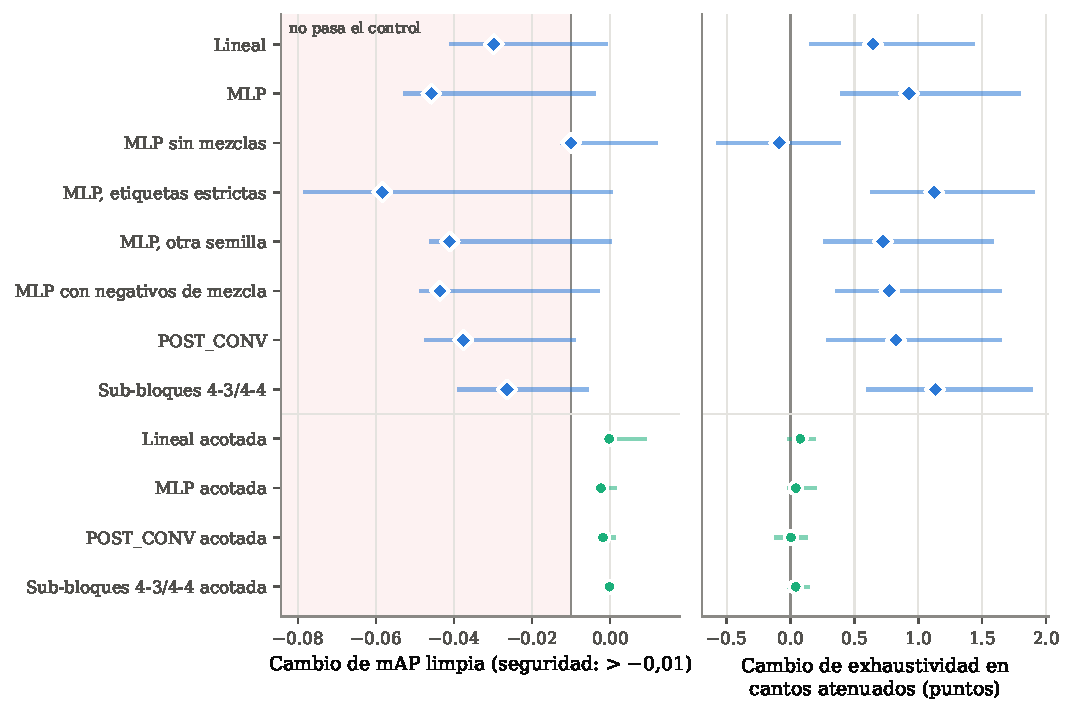
\includegraphics[width=0.92\linewidth]{fig_deep_tradeoff.pdf}
  \caption{Cambio respecto de BirdNET de cada modelo anclado, con intervalos del 95\,\%. Izquierda: mAP limpia; a la izquierda de la línea de $-0{,}01$
  no se pasa el control de seguridad. Derecha: exhaustividad media sobre cantos atenuados con el mismo volumen de alertas. Rombos: corrección libre.
  Círculos: corrección acotada.}\label{fig:deeptradeoff}
\end{figure}

\begin{figure}[H]
  \centering
  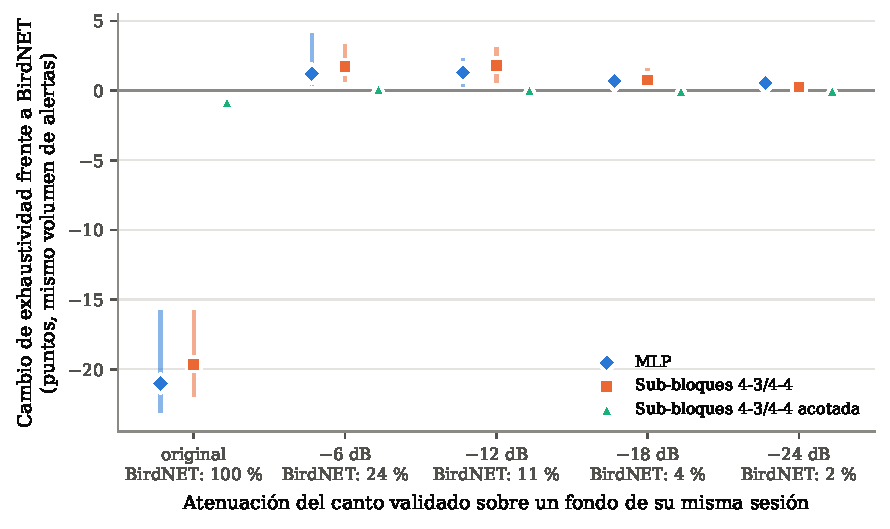
\includegraphics[width=0.88\linewidth]{fig_deep_m3.pdf}
  \caption{Cambio de exhaustividad respecto de BirdNET en cada nivel de atenuación, con el mismo volumen de alertas e intervalos del 95\,\%.
  Bajo cada nivel se indica la exhaustividad de BirdNET.}\label{fig:deepm3}
\end{figure}

\paragraph{Rechazos expertos: verificación en dos etapas.}
El segundo problema medible es descartar falsos positivos entre las propuestas de BirdNET. BirdNET deja por encima de cada rechazo, de media, el
\deepRejPctBirdnet\,\% de las detecciones validadas de su especie y grabadora (M2 = \deepRejBirdnet). Las sondas entrenadas desde cero quedan muy por
debajo de BirdNET como detectores independientes (mAP limpia \deepCleanProbeNew). En cambio, ordenan las propuestas de BirdNET mejor que él:
M2 = \deepRejProbeNew, una diferencia de \deepRejDeltaProbeNew{} con un intervalo de \deepRejCiProbeNew{} (tabla~\ref{tab:deepverifiers} y
figura~\ref{fig:deepm2}).

El esquema de dos etapas aprovecha las dos cosas: BirdNET decide qué se propone y la sonda ordena las propuestas. El conjunto de alertas es
exactamente el de BirdNET, de modo que la exhaustividad no cambia. Pasa el control de seguridad (\deepCleanDeltaTwoStage, IC \deepCleanCiTwoStage) y
mejora M2 en \deepRejDeltaTwoStage. Con un corte que conserva el 95\,\% de las detecciones validadas de cada especie, la sonda deja por debajo
\deepRejRemovedTwoStage{} de los \deepRejections{} rechazos. Con la puntuación de BirdNET serían \deepRejRemovedBirdnet. Un verificador de cinco variables
derivadas de BirdNET (su puntuación, el margen sobre la clase competidora, el contexto de la grabación) no mejora M2
(\deepRejDeltaVerifier, IC \deepRejCiVerifier): lo que separa un rechazo de una validada no está en la salida de BirdNET, sino en el \emph{embedding}.

\begin{table}[H]
  \centering\small
  \caption{Colocación de los rechazos expertos (M2) y rechazos que quedan por debajo del corte que conserva el 95\,\% de las validadas de su especie.
  D1 y D2 son las reglas de la sección~\ref{sec:protocolo}.}\label{tab:deepverifiers}
  \fittab{tab_deep_verifiers.tex}
\end{table}

\begin{figure}[H]
  \centering
  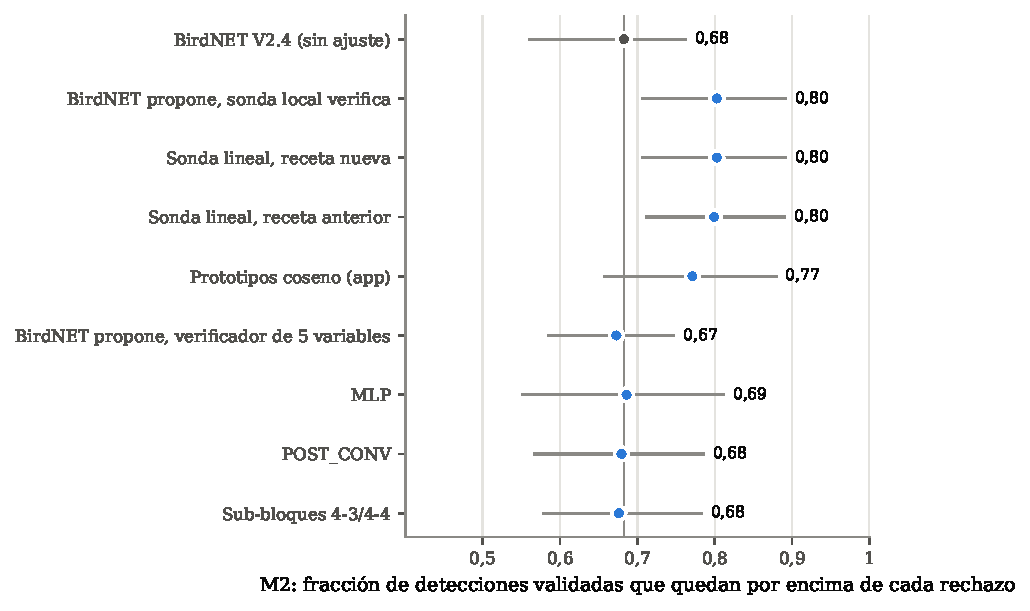
\includegraphics[width=0.88\linewidth]{fig_deep_m2.pdf}
  \caption{M2 por modelo con intervalos del 95\,\%. La línea vertical oscura marca el valor de BirdNET; 0,5 equivale a ordenar al azar.}\label{fig:deepm2}
\end{figure}

Tres cautelas. Solo hay \deepRejections{} rechazos, concentrados en pocas sesiones, y los intervalos son anchos. La mejora se mide entre sesiones
de las mismas seis grabadoras: no dice cómo se comportaría la sonda en un sitio nuevo. Y M2 compara puntuaciones de los cinco modelos de la validación
cruzada, que no están calibrados entre sí; ese ruido añadido tiende a perjudicar a la sonda, pero no se ha medido.

\paragraph{Decisión.}
Según las reglas fijadas de antemano, el esquema de dos etapas es exportable: cumple D1 y D2 sin pérdida en la exhaustividad. Las correcciones
libres cumplen D3 con una ganancia pequeña, pero no D1: no son exportables. Las acotadas cumplen D1 por construcción y no mejoran M3. Entre ellas,
la corrección lineal acotada también mejora M2 (\deepRejDeltaLinearB, IC \deepRejCiLinearB), menos de la mitad que las dos etapas, que además son más
simples. Se exporta, por tanto, el esquema de dos etapas.

\subsection{Integración del verificador}\label{sec:verificador}
La aplicación carga el verificador si encuentra el archivo \code{verificador_local.npz} junto al clasificador local. No cambia qué se detecta:
BirdNET, con la lista local y los umbrales por especie, sigue decidiendo las detecciones. El verificador añade a cada una la puntuación de la sonda y
marca como \emph{CONDESAN · revisar} las que quedan por debajo del percentil 5 de las detecciones validadas de su especie. Las especies con menos de
20 validadas no se marcan. Medido con predicciones fuera de muestra, marca el \deepFlagValid\,\% de las detecciones validadas, \deepFlagRejected{} de los
\deepFlagRejectedOf{} rechazos expertos y el \deepFlagUnreviewed\,\% de las propuestas sin revisar. Los cortes proceden de esas predicciones fuera de muestra,
mientras que la sonda que se distribuye se ajusta con todas las sesiones. En las sesiones que no intervinieron en el ajuste de sus pesos, esa sonda
marca el \deepFlagHeldValid\,\% de las validadas (\deepFlagHeldMarked{} de \deepFlagHeldOf), algo distinto del 5\,\% nominal: la marca es una ayuda para
priorizar la escucha, no un filtro. El archivo contiene los pesos de la sonda, no los de BirdNET, y no se publica en el repositorio.

\subsection{Lectura de los resultados y límites}\label{sec:lectura2}
\begin{enumerate}
  \item \textbf{El límite está en las etiquetas, no en el modelo.} Se afinaron las capas profundas de BirdNET con una pérdida adaptada al proceso de
        revisión, y la profundidad no aportó nada medible. Con estas etiquetas no se puede enseñar ni demostrar que un modelo detecta más que BirdNET, porque
        todo lo que se sabe está por encima de 0,25.
  \item \textbf{Lo que desbloquea la mejora es anotar la zona gris.} Hacen falta ventanas con puntuación de BirdNET entre 0,05 y 0,25 escuchadas por un
        experto, con presencias y ausencias. La muestra aleatoria de 300 ventanas ya preparada y la lista de ventanas en discrepancia de esta fase
        apuntan justo ahí (sección~\ref{sec:ayuda}).
  \item \textbf{La mejora validada es descartar falsos positivos}, no detectar más. Es modesta en términos absolutos, porque los expertos rechazaron pocas
        detecciones, pero es la única que estos datos permiten medir sin sesgo.
  \item \textbf{La prueba de cantos atenuados es sintética.} Atenuar un canto y sumarle un fondo no reproduce la reverberación ni el filtrado de un ave
        lejana. Sirve para comparar modelos entre sí, no para estimar cuántos cantos reales se pierden.
  \item \textbf{Cambios respecto del plan inicial.} Los dos primeros se decidieron antes de evaluar los pliegues de prueba del modelo afectado.
        (a) Se añadió una rejilla de regiones de confianza para las cabezas, porque la configuración inicial no cumplía el control en ningún pliegue interno.
        (b) La rejilla de las capas convolucionales se amplió de tres a cinco configuraciones porque los pliegues internos elegían la más agresiva, y las
        filas del clasificador pasaron a seguir la misma región de confianza. Las predicciones de la primera pasada se descartaron sin evaluarse. Aun así,
        los pliegues internos recorren entre todos el conjunto entero, de modo que esta decisión no es del todo independiente de los pliegues de prueba
        y puede favorecer ligeramente a los escalones convolucionales.
        (c) La corrección acotada y la ablación con negativos certificados se añadieron después de ver los resultados de las cabezas, y se presentan
        como análisis posteriores.
        (d) Una revisión independiente del código, hecha con los resultados ya a la vista, encontró dos defectos en el cálculo de M3. En las réplicas de
        bootstrap, una ventana de una sesión no remuestreada podía fijar el umbral; y el umbral se elegía de modo que el modelo nunca superara el volumen
        de alertas de BirdNET, lo que le dejaba algo menos (un 2\,\% de media en el escalón de los sub-bloques). Se corrigieron ambos: ahora el
        volumen se iguala exactamente. Los valores de $S$ cambiaron menos de 0,05 puntos, pero los intervalos se estrecharon, y D3 pasó de \emph{no} a
        \emph{sí} para la corrección lineal y para \code{POST_CONV}, cuyos intervalos antes rozaban el cero ($[-0{,}1;\ +1{,}3]$ y $[-0{,}0;\ +1{,}6]$ puntos).
        Ninguna decisión cambia. La selección anidada se hizo con el cálculo anterior y no se repitió. La misma revisión no encontró fugas de
        información entre pliegues en el entrenamiento.
\end{enumerate}

